\subsubsection{Markov Decision Process}
The interaction of a learner to achieve a goal can be modeled mathematically through a \textit{Markov Decision Process} (or \textit{MDP}) \cite{bible}. This allows statements about learning algorithms to be theoretically proven, such as the convergence of an agent's policy to its optimum.

We start by defining that the learning and acting instance is called the \textit{agent}, whereas its surroundings, which are delivering situations, responding to the agents actions and controlling the reward signal, are called the \textit{environment}. The agent therefore strives to maximize its rewards by performing actions based on previously perceived situations. 

In Markov Decision Processes, the agent-environment interaction only occurs at discrete timesteps $t \in \{0, 1, 2, ...\}$. At each timestep $t$, the environment provides a \textit{state} $S_t \in \mathscr{S}$ to the agent, where $\mathscr{S}$ is the set of all possible states. Based on this state, the agent may select an \textit{action} $A_t \in \mathscr{A}(S_t)$, with $\mathscr{A}(S_t)$ being the set of legal actions in state $S_t$. As a result of this action, the agent receives a \textit{reward} $R_t \in \mathscr{R} \subset \mathbb{R}$. Note that this means there is no reward associated with the very first timestep. A sequence following this pattern of states, actions and rewards is called a \textit{trajectory}. This process is visualized in figure \ref{fig:mdp_visualization}.

\begin{figure}[ht]
    \centering
    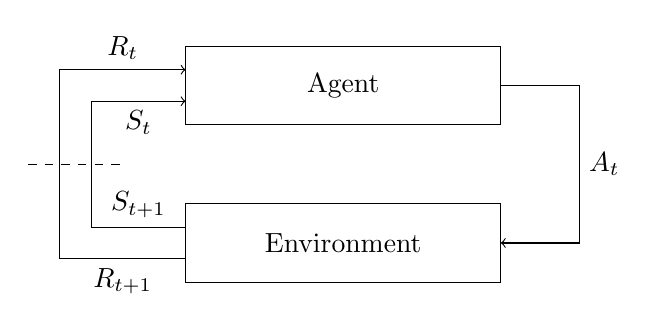
\begin{tikzpicture}
        \draw (0, 2) rectangle node {Agent} (4, 3);
        \draw (0, 0) rectangle node {Environment} (4, 1);

        \draw [->] (4, 2.5) -- (5, 2.5) -- node[right] {$A_t$} (5, 0.5) -- (4, 0.5);

        \draw [->] (0, 0.3) -- node[below] {$R_{t+1}$} (-1.6, 0.3) -- (-1.6, 2.7) --node[above] {$R_t$}  (0, 2.7);
        \draw [->] (0, 0.7) -- node[above] {$S_{t+1}$} (-1.2, 0.7) -- (-1.2, 2.3) -- node[below] {$S_t$} (0, 2.3);

        \draw [dashed] (-2, 1.5) -- (-0.8, 1.5);
    \end{tikzpicture}
    \caption{Visualization of the feedback loop in a Markov Decision Process.}
    \label{fig:mdp_visualization}
\end{figure}

In a \textit{finite Markov Decision Process} \cite{bible}, the sets of states $\mathscr{S}$, actions $\mathscr{A}(s) : \forall s \in \mathscr{S}$ and rewards $\mathscr{R}$ are all finite. With this constraint, we can use the function $p : \mathscr{S} \times \mathscr{R} \times \mathscr{S} \times \mathscr{A} \mapsto \left[0, 1\right]$ to denote probabilities of state transitions occuring. For example, $p\left(s', r \given s, a\right)$ refers to the probability of seeing state $s'$ and receiving reward $r$ after taking action $a$ in state $s$. This implies that transition probabilities are only dependant on the current state and action, not on past information.

An agent should not focus solely on choosing the action $A_t$ which results in the highest \textit{immediate reward} $R_{t+1}$. Instead, future rewards should also be taken into consideration. Formally, we define the \textit{return}, which is the sum of all rewards at subsequent timesteps until the final timestep $T$.
\begin{equation*}
    G_t = R_{t+1} + R_{t+2} + R_{t+3} + ... + R_T
\end{equation*}
Accordingly, an agent aims to maximize the expected return at each step. The concept of a final timestep only applies for tasks which have a clearly defined beginning and end, i.e. are repetitive in nature. We call a single cycle of these repetitive tasks \textit{episode}.

For tasks which can potentially continue indefinitely, i.e. $T = \infty$, $G_t$ may also become infinite. To avoid this issue, we introduce a \textit{discount rate} (or \textit{discount factor}) $\gamma \in [0, 1]$, and define the \textit{discounted return} as follows:
\begin{equation*}
    G_t = R_{t+1} + \gamma R_{t+2} + \gamma^2 R_{t+3} + ...
        = \sum_{k=t+1}^T \gamma^{k-t-1} R_k
\end{equation*}
The parameter $\gamma$ determines to what extend the agent prefers rewards in the near over those in the far future. As an example, an agent with $\gamma = 0$ cares only about the immediate reward, whereas the same agent with $\gamma = 0.99$ will optimize for a large time window of rewards. Choosing $\gamma < 1$ ensures that $G_t$ will not become infinite.

In some cases, it is not realistic for the agent to receive the full state of the environment. For example, a robot with a camera cannot possibly measure all physical properties of its surroundings at all times. While a well defined \textit{latent state} may exist, it only retrieves an \textit{observation} produced by this state instead. These types of environments are modeled as \textit{Partially Observable Markov Decision Processes}, or \textit{POMDPs} \cite{bible}.